\documentclass[11pt,a4paper]{article}

\usepackage[utf8]{inputenc}
\usepackage[margin=0.85in]{geometry}
\usepackage{amsmath,amssymb,amsfonts}
\usepackage{graphicx}
\usepackage{xcolor}
\usepackage{subcaption}
\usepackage{float}
\usepackage{hyperref}
\usepackage{booktabs}
\usepackage{microtype}
\usepackage{tabularx}
\usepackage{array}

\hypersetup{
    colorlinks=true,
    linkcolor=blue!70!black,
    citecolor=blue!70!black,
    urlcolor=blue!70!black
}

\title{\textbf{\Large Part 2: User-Guided Region Segmentation and GrabCut}}
\author{}
\date{}

\begin{document}
\maketitle

GrabCut extends graph-cut segmentation into an iterative, user-guided method for extracting foreground objects. It initializes foreground and background appearance models from a bounding rectangle, then alternates between graph-cut labeling and model re-estimation. We study four approaches, progressing from pixel-wise classification to iterative segmentation:

\begin{enumerate}
    \item \textbf{Maximum Likelihood Classification:} Fit 3D Gaussian color models to marked seeds and classify pixels by their relative likelihoods.
    \item \textbf{K-means Clustering:} Cluster pixels into two color classes using seed means for initialization, while keeping seed labels fixed and tracking WCSS.
    \item \textbf{Graph Cuts:} Minimize an energy defined by regional likelihoods and pairwise boundary penalties on a 4-connected graph, using SciPy's maximum-flow algorithm. We also study the effects of $\lambda$ and $\sigma$.
    \item \textbf{GrabCut-like Segmentation:} Alternate between Gaussian model estimation and graph-cut labeling, initialized using a single bounding rectangle.
\end{enumerate}

\begin{figure}[H]
    \centering
    \begin{subfigure}[b]{0.48\textwidth}
        \centering
        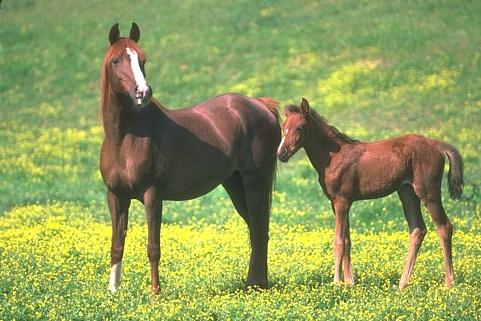
\includegraphics[width=\linewidth]{image2/input.jpg}
        \caption{Original input image (BSDS300 \#113044)}
    \end{subfigure}
    \hfill
    \begin{subfigure}[b]{0.48\textwidth}
        \centering
        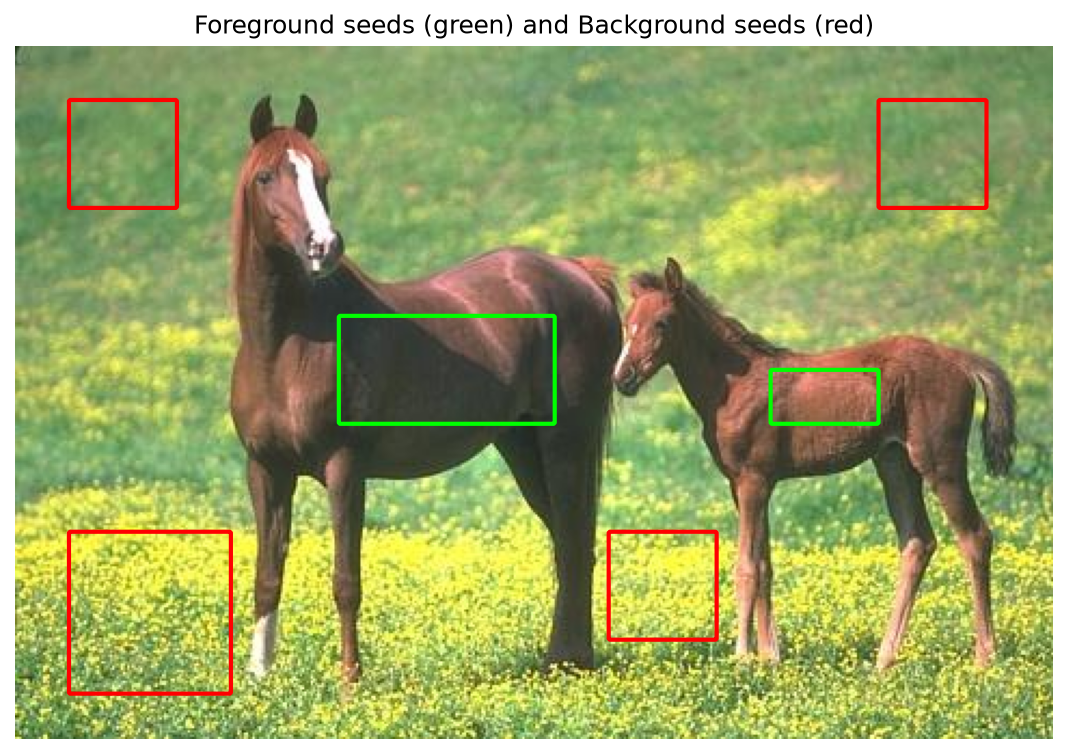
\includegraphics[width=\linewidth]{image2/seed_selection.png}
        \caption{Foreground (green) and background (red) seeds}
    \end{subfigure}
    \caption{Input image of two grazing horses and the seed regions used to fit the color models.}
    \label{fig:input_and_seeds}
\end{figure}

\section{Image Selection and Seed Specification}

We selected BSDS300 image \#113044, which depicts two brown horses grazing in a green pasture. The contrast between the horses' brown coats and the green grass makes the image suitable for color-based segmentation.

The image was resized to $512 \times 341$ pixels for pixel-wise clustering and to $180 \times 120$ pixels for graph-cut stages to reduce the cost of sparse max-flow operations. We marked two foreground subrectangles on the horses and four background subrectangles across different grass patches.

\section{Part (a): Maximum Likelihood Classification}

\subsection{Multivariate Gaussian Appearance Model}

Each RGB pixel $\mathbf{x}=(R,G,B)^T\in\mathbb{R}^3$ is modeled using a class-conditional Gaussian distribution $\mathcal{N}(\boldsymbol{\mu}_k,\boldsymbol{\Sigma}_k)$, where $k\in\{\text{FG},\text{BG}\}$:

\[
P(\mathbf{x}\mid k)=
\frac{1}{(2\pi)^{3/2}|\boldsymbol{\Sigma}_k|^{1/2}}
\exp\left(
-\frac{1}{2}(\mathbf{x}-\boldsymbol{\mu}_k)^T
\boldsymbol{\Sigma}_k^{-1}(\mathbf{x}-\boldsymbol{\mu}_k)
\right).
\]

The mean and covariance are estimated from the marked seed pixels $\mathcal{S}_k$:

\[
\boldsymbol{\mu}_k=\frac{1}{|\mathcal{S}_k|}
\sum_{\mathbf{x}\in\mathcal{S}_k}\mathbf{x},
\qquad
\boldsymbol{\Sigma}_k=\frac{1}{|\mathcal{S}_k|-1}
\sum_{\mathbf{x}\in\mathcal{S}_k}
(\mathbf{x}-\boldsymbol{\mu}_k)(\mathbf{x}-\boldsymbol{\mu}_k)^T.
\]

We add ridge regularization, $\epsilon\mathbf{I}$ with $\epsilon=25.0$, to the covariance diagonal to ensure numerical stability and positive definiteness. The resulting log-likelihood is

\[
\ln P(\mathbf{x}\mid k)=
-\frac{1}{2}\left[
(\mathbf{x}-\boldsymbol{\mu}_k)^T\boldsymbol{\Sigma}_k^{-1}
(\mathbf{x}-\boldsymbol{\mu}_k)
+\ln|\boldsymbol{\Sigma}_k|+3\ln(2\pi)
\right].
\]

\subsection{Likelihood Visualization and Classification}

Figure below shows the normalized likelihood maps. The foreground model assigns high likelihood to the horses and low likelihood to the grass, while the background model assigns high likelihood across the pasture.

\begin{figure}[H]
    \centering
    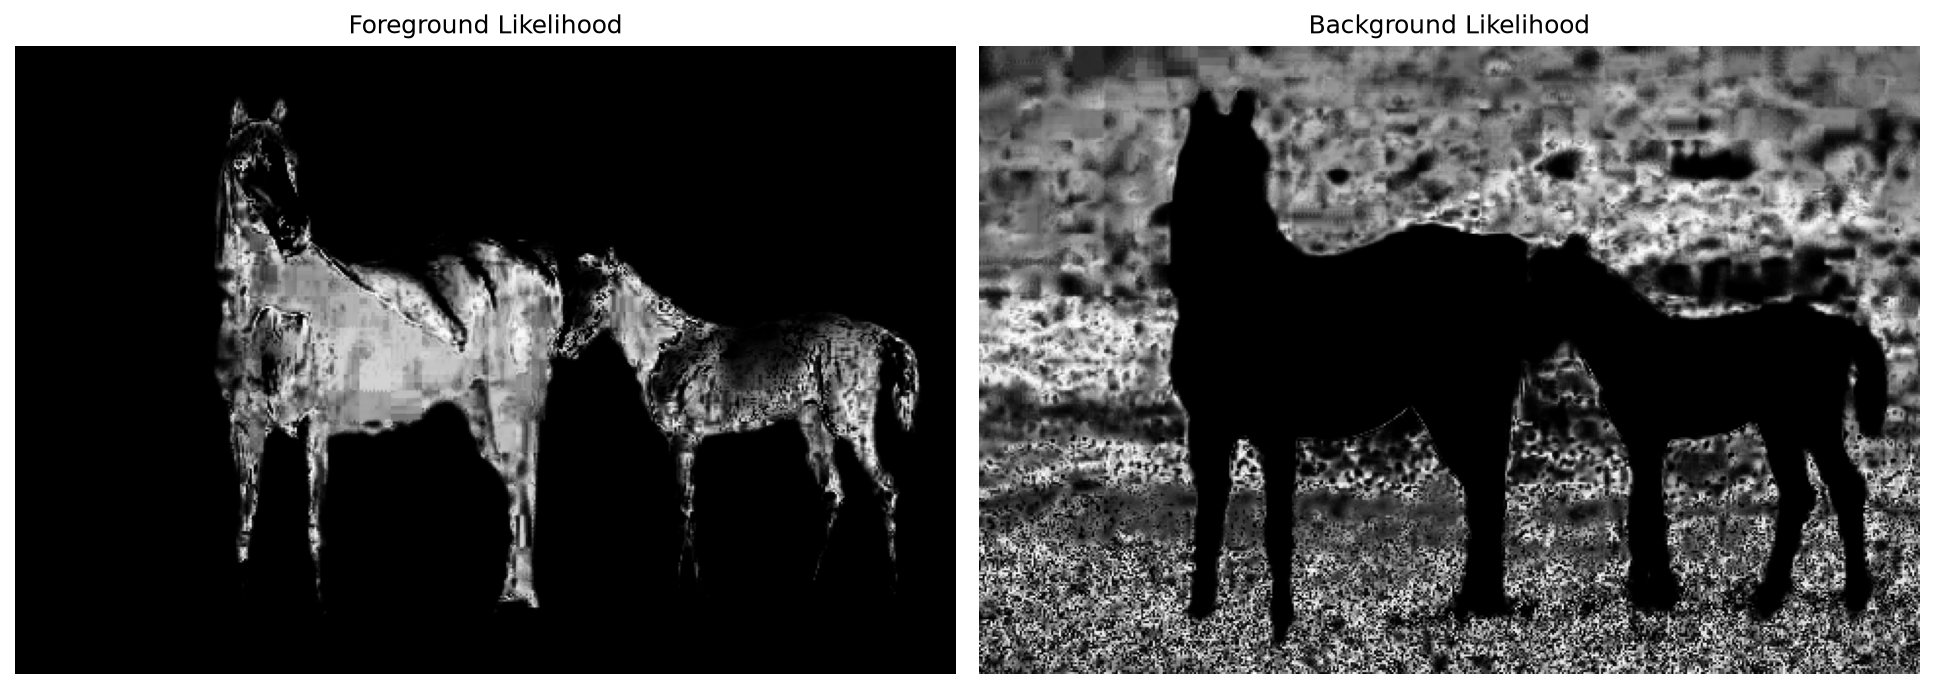
\includegraphics[width=0.9\linewidth]{image2/likelihood.png}
    \caption{Pixel-wise foreground likelihood $P(\mathbf{x}\mid\text{FG})$ (left) and background likelihood $P(\mathbf{x}\mid\text{BG})$ (right).}
    \label{fig:likelihood}
\end{figure}

With a uniform prior, each pixel is assigned to the class with the higher log-likelihood:
\[
\ln P(\mathbf{x}\mid\text{FG}) >
\ln P(\mathbf{x}\mid\text{BG})
\quad\Rightarrow\quad
\text{foreground}.
\]
Marked seeds retain their assigned labels.

Figure below shows the resulting segmentation. Each pixel is replaced by its class mean color, and the class boundary is highlighted in red. The method captures the horses' overall shapes but produces isolated false positives in shadowed grass because it does not enforce spatial consistency.

\begin{figure}[H]
    \centering
    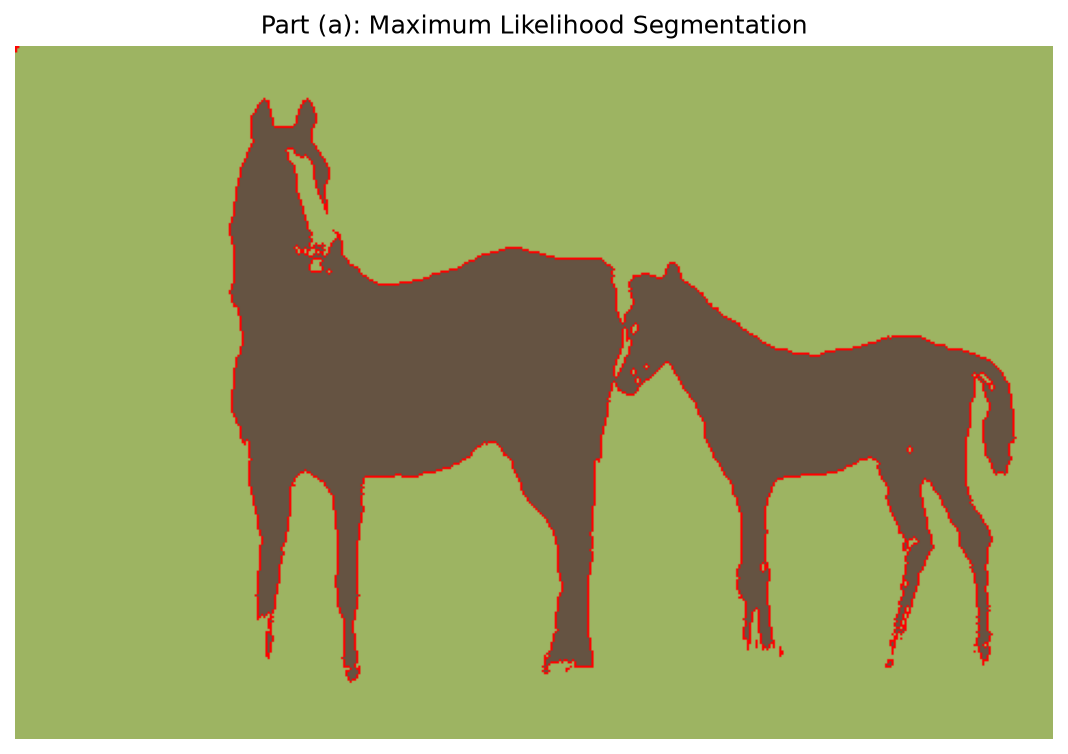
\includegraphics[width=0.42\linewidth]{image2/likelihood_segmentation.png}
    \caption{Part (a): Maximum-likelihood segmentation, with pixels replaced by their class mean colors and the boundary highlighted in red.}
    \label{fig:ml_seg}
\end{figure}

\section{Part (b): K-means Clustering}

\subsection{Formulation and Seed Initialization}

K-means partitions the pixels into $K=2$ clusters by minimizing the within-cluster sum of squares (WCSS):

\[
\mathrm{WCSS}=
\sum_{k=0}^{1}\sum_{\mathbf{x}_i\in\mathcal{C}_k}
\|\mathbf{x}_i-\boldsymbol{\mu}_k\|_2^2.
\]

We initialize the cluster centers with the mean colors of the foreground and background seeds:

\[
\boldsymbol{\mu}_0^{(0)}
=\frac{1}{|\mathcal{S}_{\mathrm{FG}}|}
\sum_{\mathbf{x}\in\mathcal{S}_{\mathrm{FG}}}\mathbf{x},
\qquad
\boldsymbol{\mu}_1^{(0)}
=\frac{1}{|\mathcal{S}_{\mathrm{BG}}|}
\sum_{\mathbf{x}\in\mathcal{S}_{\mathrm{BG}}}\mathbf{x}.
\]



\subsection{Convergence and WCSS Analysis}



\begin{figure}[H]
    \centering
    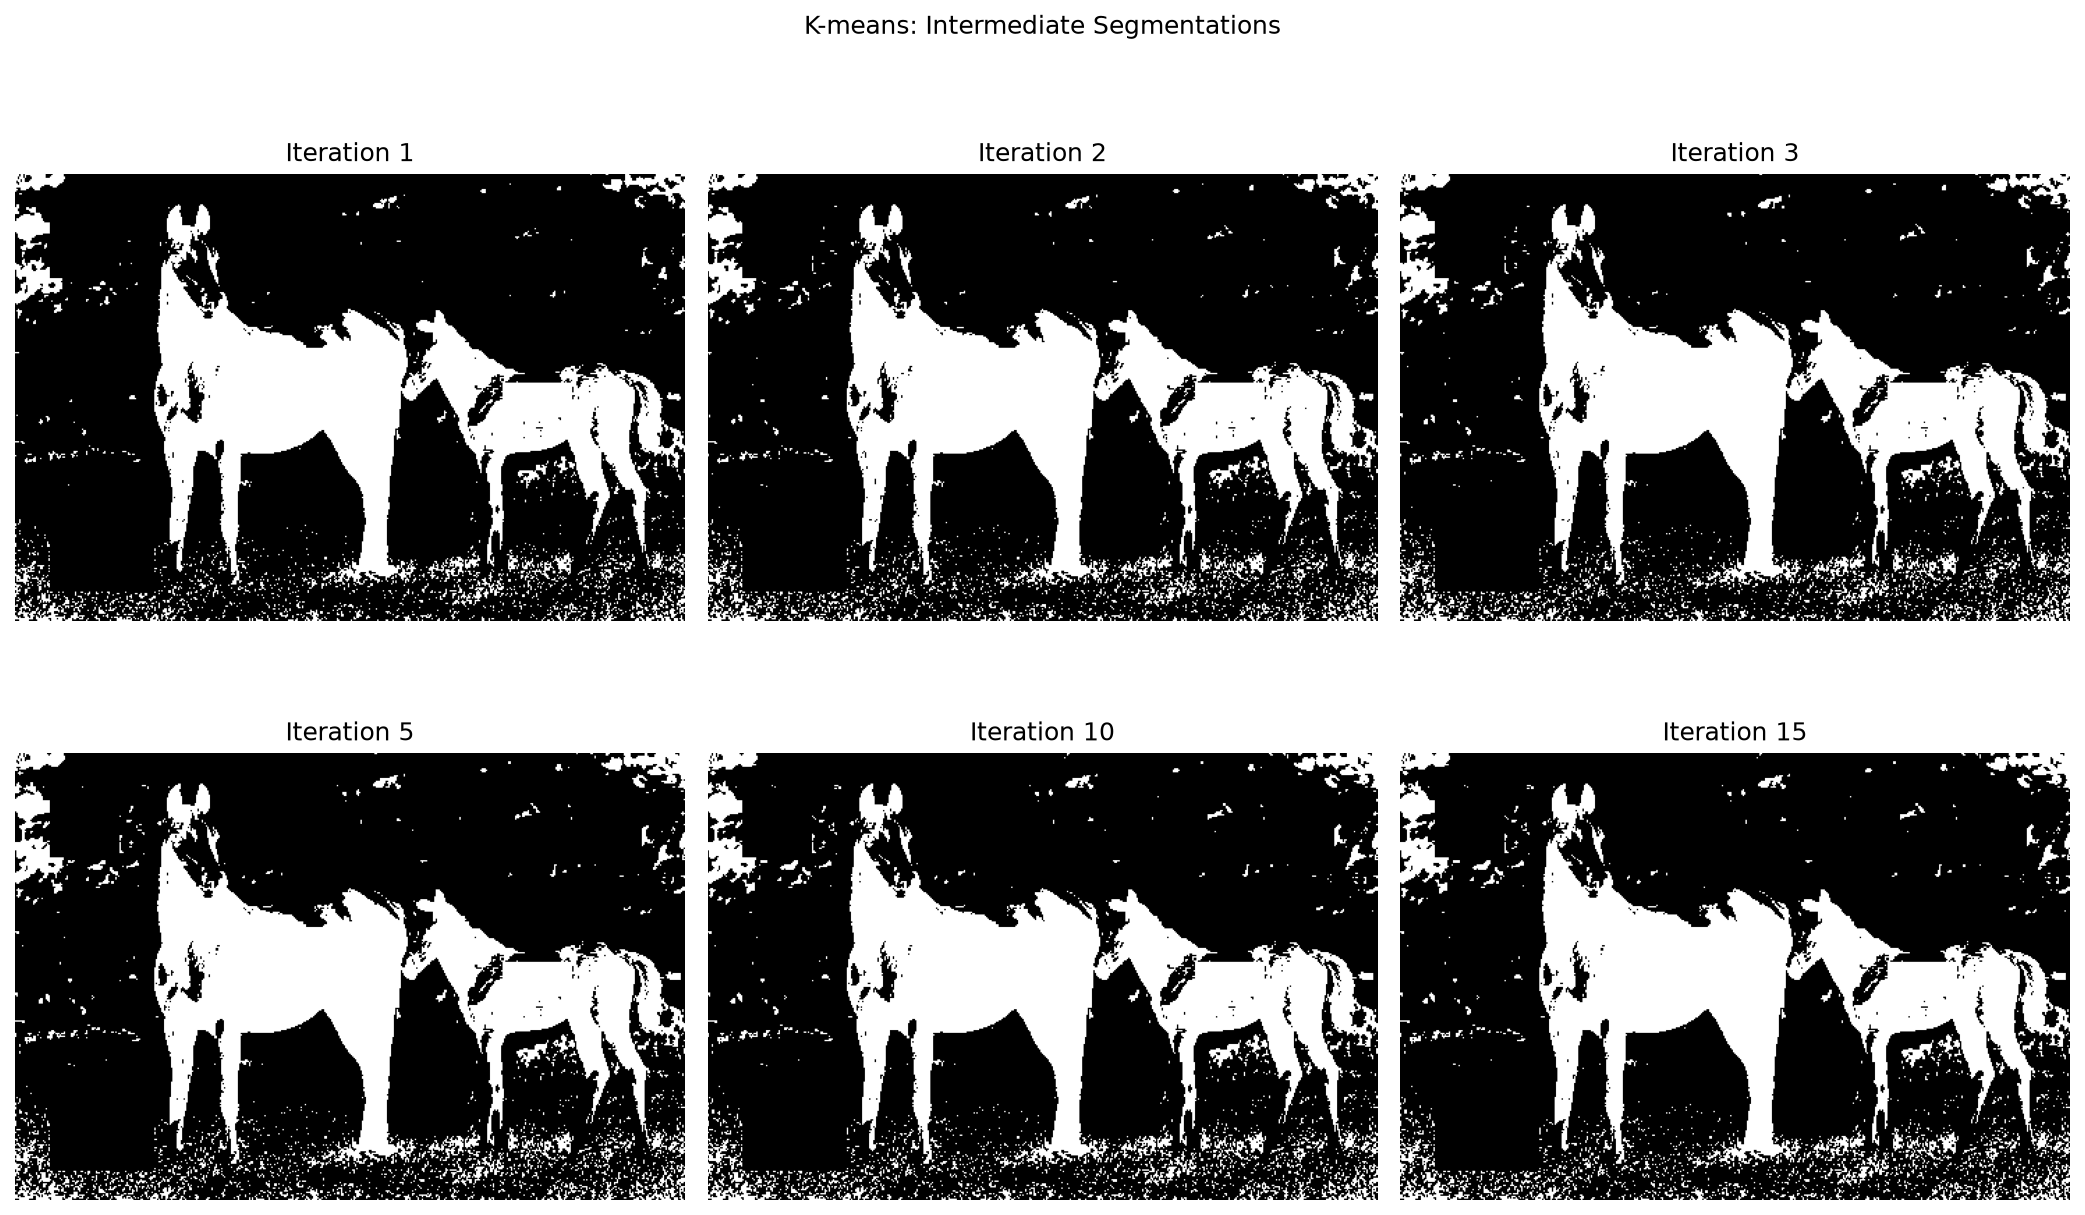
\includegraphics[width=0.90\linewidth]{image2/intermediate_segmentation.png}
    \caption{Part (b): K-means segmentation masks at iterations 1, 2, 3, 5, 10, and 15.}
    \label{fig:kmeans_snapshots}
\end{figure}
Each iteration assigns pixels to the nearest cluster center and recomputes the centers. Figure above shows the assignments at iterations 1, 2, 3, 5, 10, and 15. The boundaries stabilize within the first five iterations.
As shown in Figure below, WCSS decreases monotonically from $4.68\times10^8$ at iteration 1 to a plateau of $3.57\times10^8$ by iteration 10, indicating convergence.

The final segmentation separates the two color classes more sharply than maximum likelihood classification. However, it still contains isolated noisy pixels because it does not model spatial relationships.

\begin{figure}[H]
    \centering
    \begin{subfigure}[b]{0.48\textwidth}
        \centering
        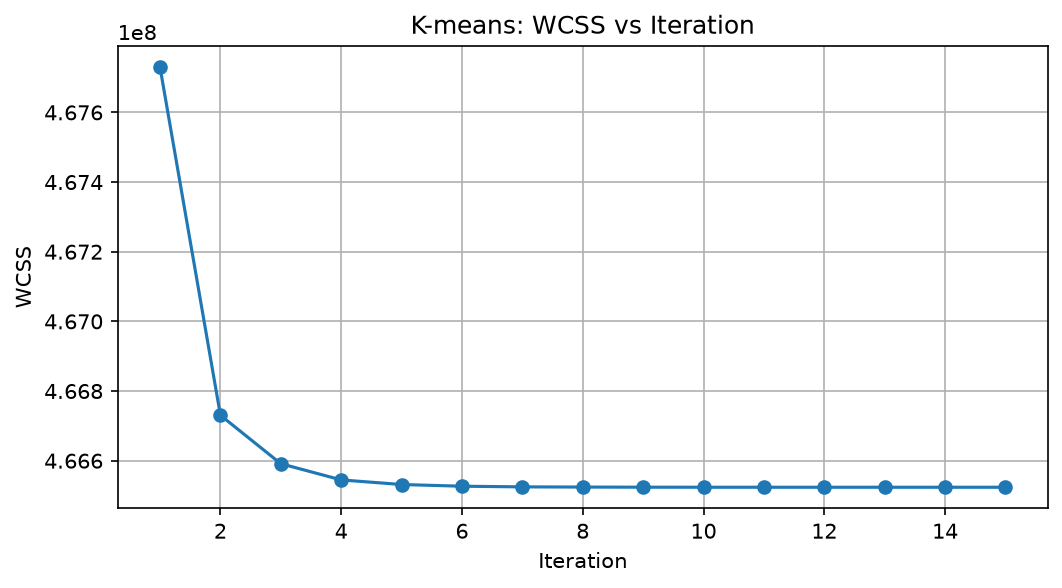
\includegraphics[width=\linewidth]{image2/K_means_graph.png}
        \caption{WCSS versus iteration}
        \label{fig:kmeans_graph}
    \end{subfigure}
    \hfill
    \begin{subfigure}[b]{0.48\textwidth}
        \centering
        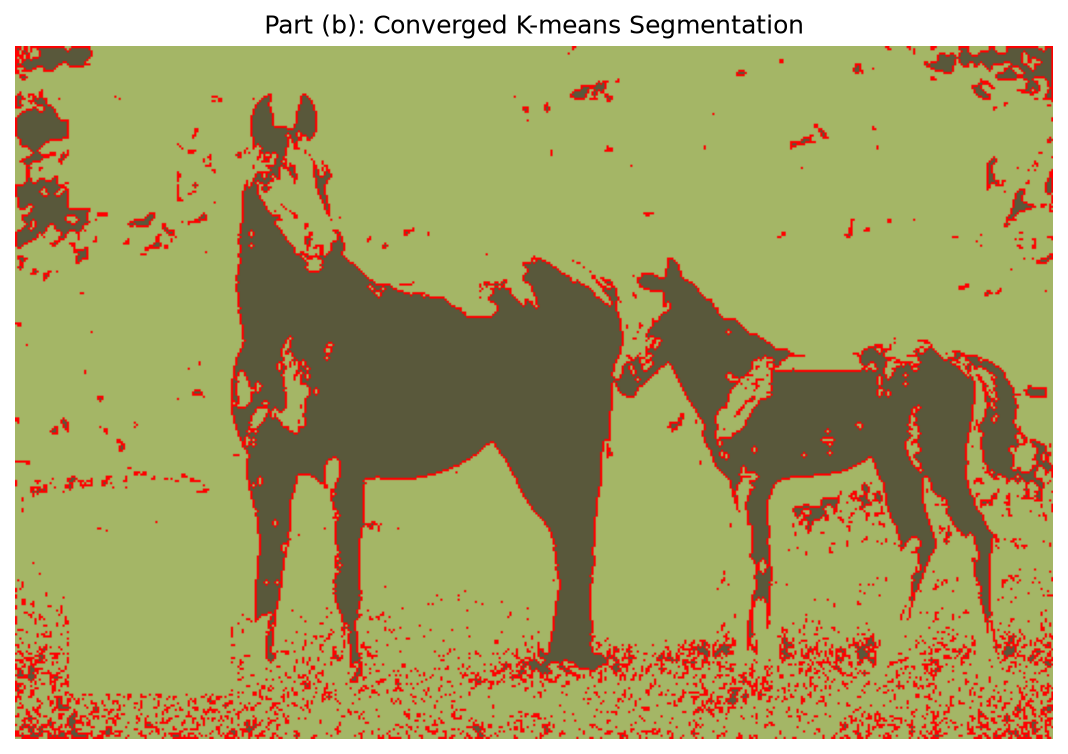
\includegraphics[width=\linewidth]{image2/converged_K_mean_segmentation.png}
        \caption{Converged K-means segmentation}
        \label{fig:kmeans_converged}
    \end{subfigure}
    \caption{K-means convergence: (a) WCSS curve and (b) final segmentation with boundaries highlighted in red.}
\end{figure}

\section{Part (c): Graph Cut Segmentation via Max-Flow}

\subsection{Energy Minimization Framework}

Maximum likelihood and K-means classify pixels independently. To enforce spatial consistency, we formulate segmentation as binary Markov random field (MRF) energy minimization on a 4-connected graph:

\[
E(\mathbf{L})=
\sum_{p\in V}D_p(L_p)+
\sum_{(p,q)\in E}V_{p,q}(L_p,L_q),
\]
where $L_p\in\{0,1\}$ denotes the background or foreground label.

\paragraph{Regional penalties (t-links).}
The data costs are the negative log-likelihoods of the Gaussian models fitted in Part (a):

\[
D_p(\mathrm{FG})=-\ln P(\mathbf{x}_p\mid\mathrm{FG}),
\qquad
D_p(\mathrm{BG})=-\ln P(\mathbf{x}_p\mid\mathrm{BG}).
\]

For numerical stability, we subtract
$\min(D_p(\mathrm{FG}),D_p(\mathrm{BG}))$ from both costs at each pixel. Seed labels are enforced using hard constraints: set $D_p(\mathrm{FG})=\infty$ for known background pixels and $D_p(\mathrm{BG})=\infty$ for known foreground pixels. The source-to-pixel capacity is $D_p(\mathrm{BG})$, and the pixel-to-sink capacity is $D_p(\mathrm{FG})$.

\paragraph{Boundary penalties (n-links).}
For each pair of 4-connected neighbors, the edge capacity penalizes cuts between similar-colored pixels:

\[
V_{p,q}=
\lambda\exp\left(
-\frac{\|\mathbf{x}_p-\mathbf{x}_q\|_2^2}{2\sigma^2}
\right).
\]

The penalty approaches $\lambda$ when neighboring colors are similar, discouraging a boundary between them. It decreases across strong color edges, allowing the cut to follow likely object boundaries.

\subsection{Min-Cut Computation and Result}

We compute the minimum cut using SciPy's sparse maximum-flow routine. Pixels reachable from the source in the residual graph are assigned to the foreground.

Figure below shows the result for the selected parameters, $\lambda=3.5$ and $\sigma=25.0$. The pairwise smoothness term removes the isolated noise seen in Parts (a) and (b), producing more coherent horse silhouettes.

\begin{figure}[H]
    \centering
    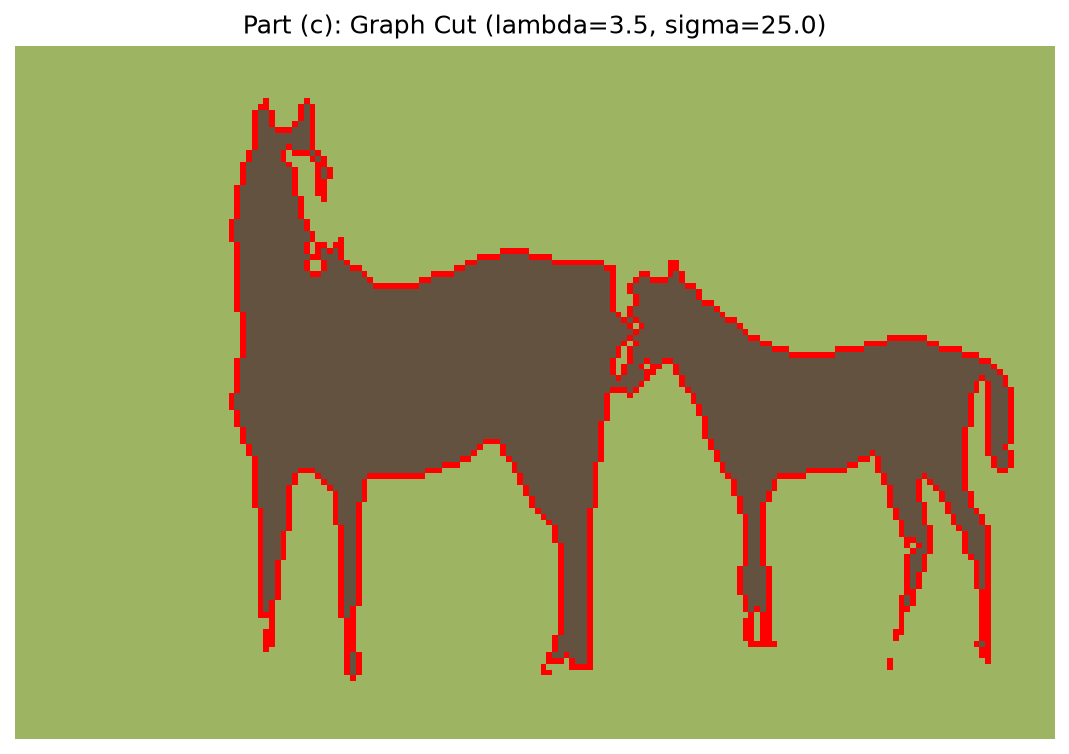
\includegraphics[width=0.62\linewidth]{image2/graph_cut.png}
    \caption{Part (c): Graph-cut segmentation with $\lambda=3.5$ and $\sigma=25.0$.}
    \label{fig:graph_cut_default}
\end{figure}

\subsection{Parameter Sensitivity: $\lambda$ and $\sigma$}

We varied the smoothness weight $\lambda$ and contrast parameter $\sigma$ to examine their effects on segmentation.

\subsubsection{Effect of Smoothness Weight $\lambda$}

Figure below compares $\lambda=0.35$ and $\lambda=35.0$, with $\sigma=25.0$ fixed:

\begin{itemize}
    \item \textbf{Small $\lambda=0.35$:} The smoothness penalty is weak, so the data term dominates and isolated noisy regions reappear in the background.
    \item \textbf{Large $\lambda=35.0$:} The strong penalty favors shorter boundaries, causing over-smoothing, boundary shrinkage, and erosion of thin structures such as the horses' legs.
\end{itemize}

\begin{figure}[H]
    \centering
    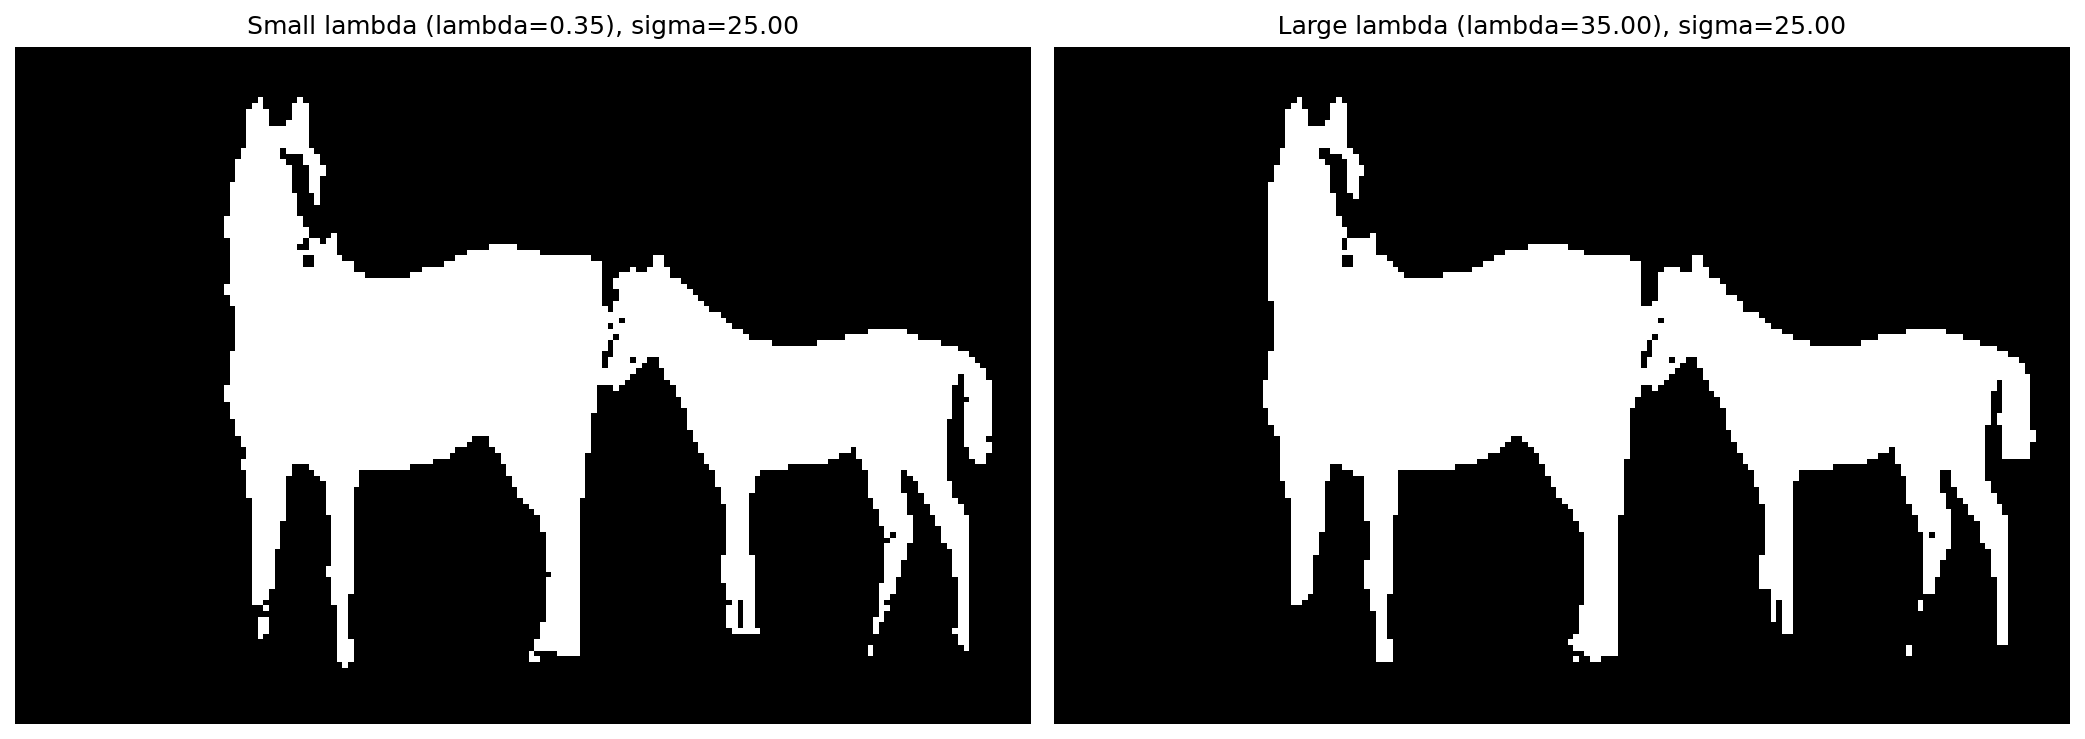
\includegraphics[width=0.88\linewidth]{image2/graph_cut_lambda.png}
    \caption{Effect of $\lambda$: a small value ($0.35$, left) produces noisy fragments, while a large value ($35.0$, right) over-smooths and shrinks the boundary.}
    \label{fig:gc_lambda}
\end{figure}

\subsubsection{Effect of Color Contrast Sensitivity $\sigma$}

Figure below compares $\sigma=8.33$ and $\sigma=75.0$, with $\lambda=3.5$ fixed:

\begin{itemize}
    \item \textbf{Small $\sigma=8.33$:} The exponential penalty decays rapidly. Even small color differences between neighboring grass pixels reduce the penalty substantially, allowing cuts within otherwise uniform regions.
    \item \textbf{Large $\sigma=75.0$:} The penalty remains high even across genuine color edges. Consequently, the cut is less sensitive to object contours and produces over-smoothed boundaries.
\end{itemize}

\begin{figure}[H]
    \centering
    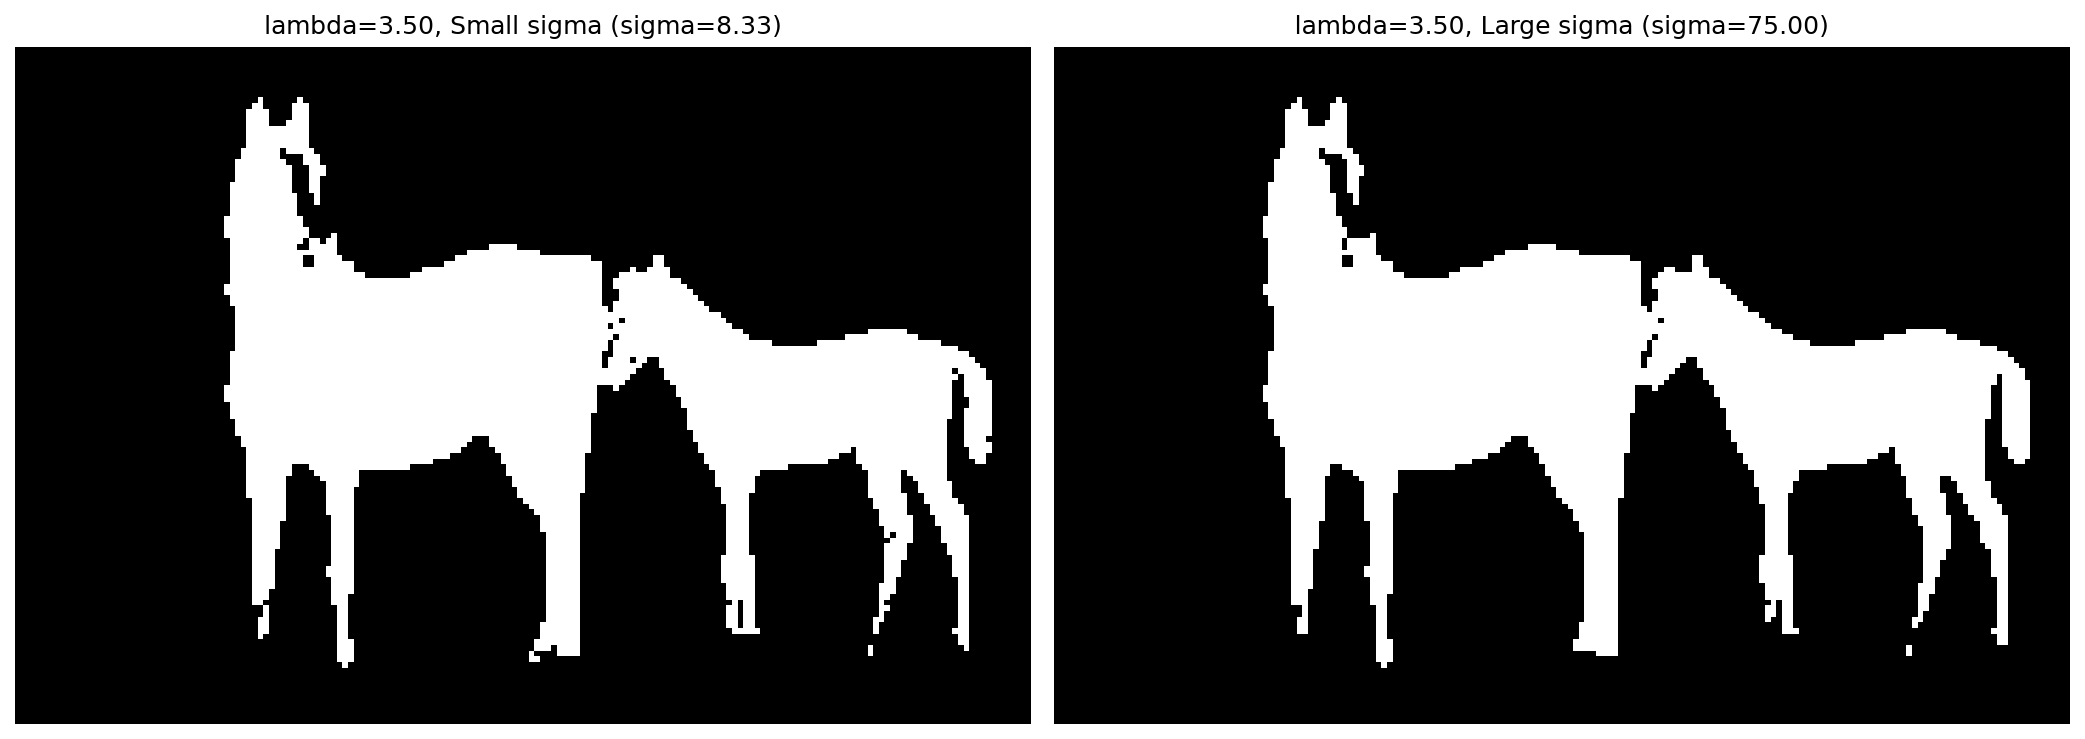
\includegraphics[width=0.88\linewidth]{image2/graph_cut_sigma.png}
    \caption{Effect of $\sigma$: a small value ($8.33$, left) causes fragmentation, while a large value ($75.0$, right) over-smooths boundaries across color transitions.}
    \label{fig:gc_sigma}
\end{figure}

\section{Part (d): GrabCut-like Iterative Approach}

\subsection{Rectangle-Based Initialization}

Unlike Parts (a)--(c), which require manually marked foreground and background regions, GrabCut starts with a single bounding rectangle around the objects.

\begin{figure}[H]
    \centering
    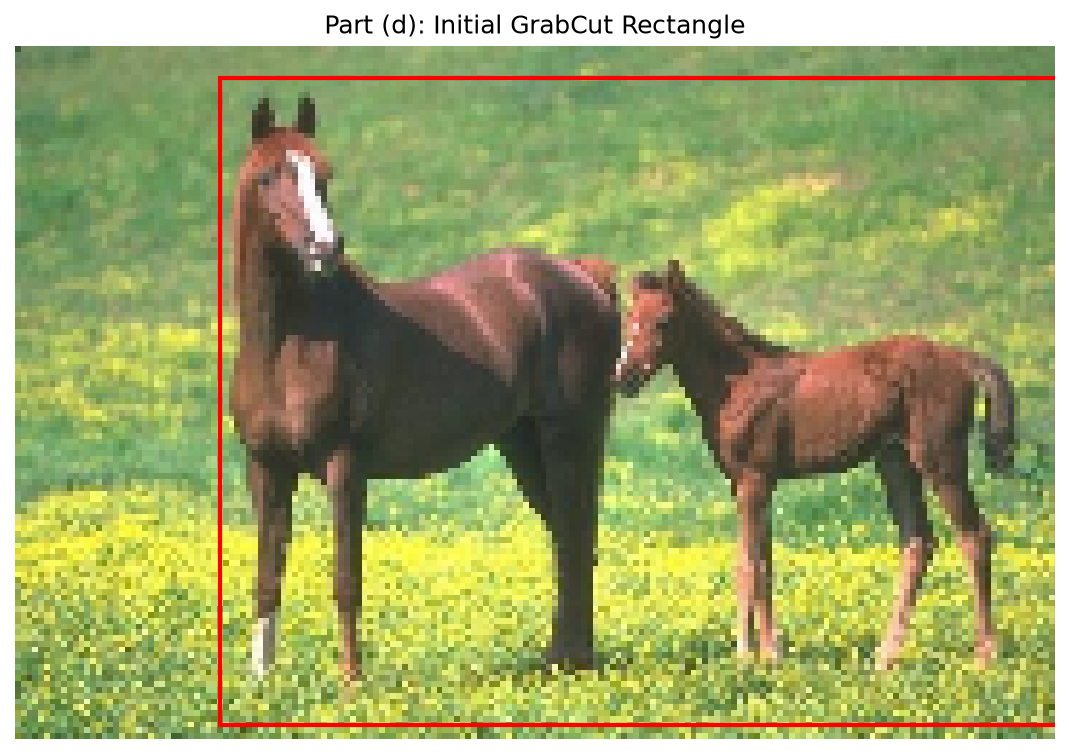
\includegraphics[width=0.55\linewidth]{image2/grab_cut_rect.png}
    \caption{Part (d): User-defined bounding rectangle (red) enclosing both horses.}
    \label{fig:grabcut_rect}
\end{figure}

Initialization assigns pixels outside the rectangle to definite background ($T_B$), enforcing this label with $D_p(\mathrm{FG})=\infty$. Pixels inside the rectangle are initialized as probable foreground ($T_F$). The eroded rectangle interior supplies the initial foreground color samples, while pixels outside the rectangle supply the background samples.

\subsection{Alternating Optimization}

The algorithm performs six iterations, alternating between:

\begin{enumerate}
    \item \textbf{Graph cut (E-step):} Using the current Gaussian parameters, solve the min-cut on the 4-connected grid to label pixels inside the rectangle as foreground or background.
    \item \textbf{Model estimation (M-step):} Re-estimate the foreground and background means, $\boldsymbol{\mu}_k$, and covariances, $\boldsymbol{\Sigma}_k$, from the updated labels.
\end{enumerate}

Figure shows the masks over iterations 1--6. Initially, most of the rectangle interior is labeled foreground. In iterations 2 \& 3, the background model learns the grass within the rectangle, enabling the graph cut to remove it and isolate the horses.The segmentation stabilizes by iteration 5.

\begin{figure}[H]
    \centering
    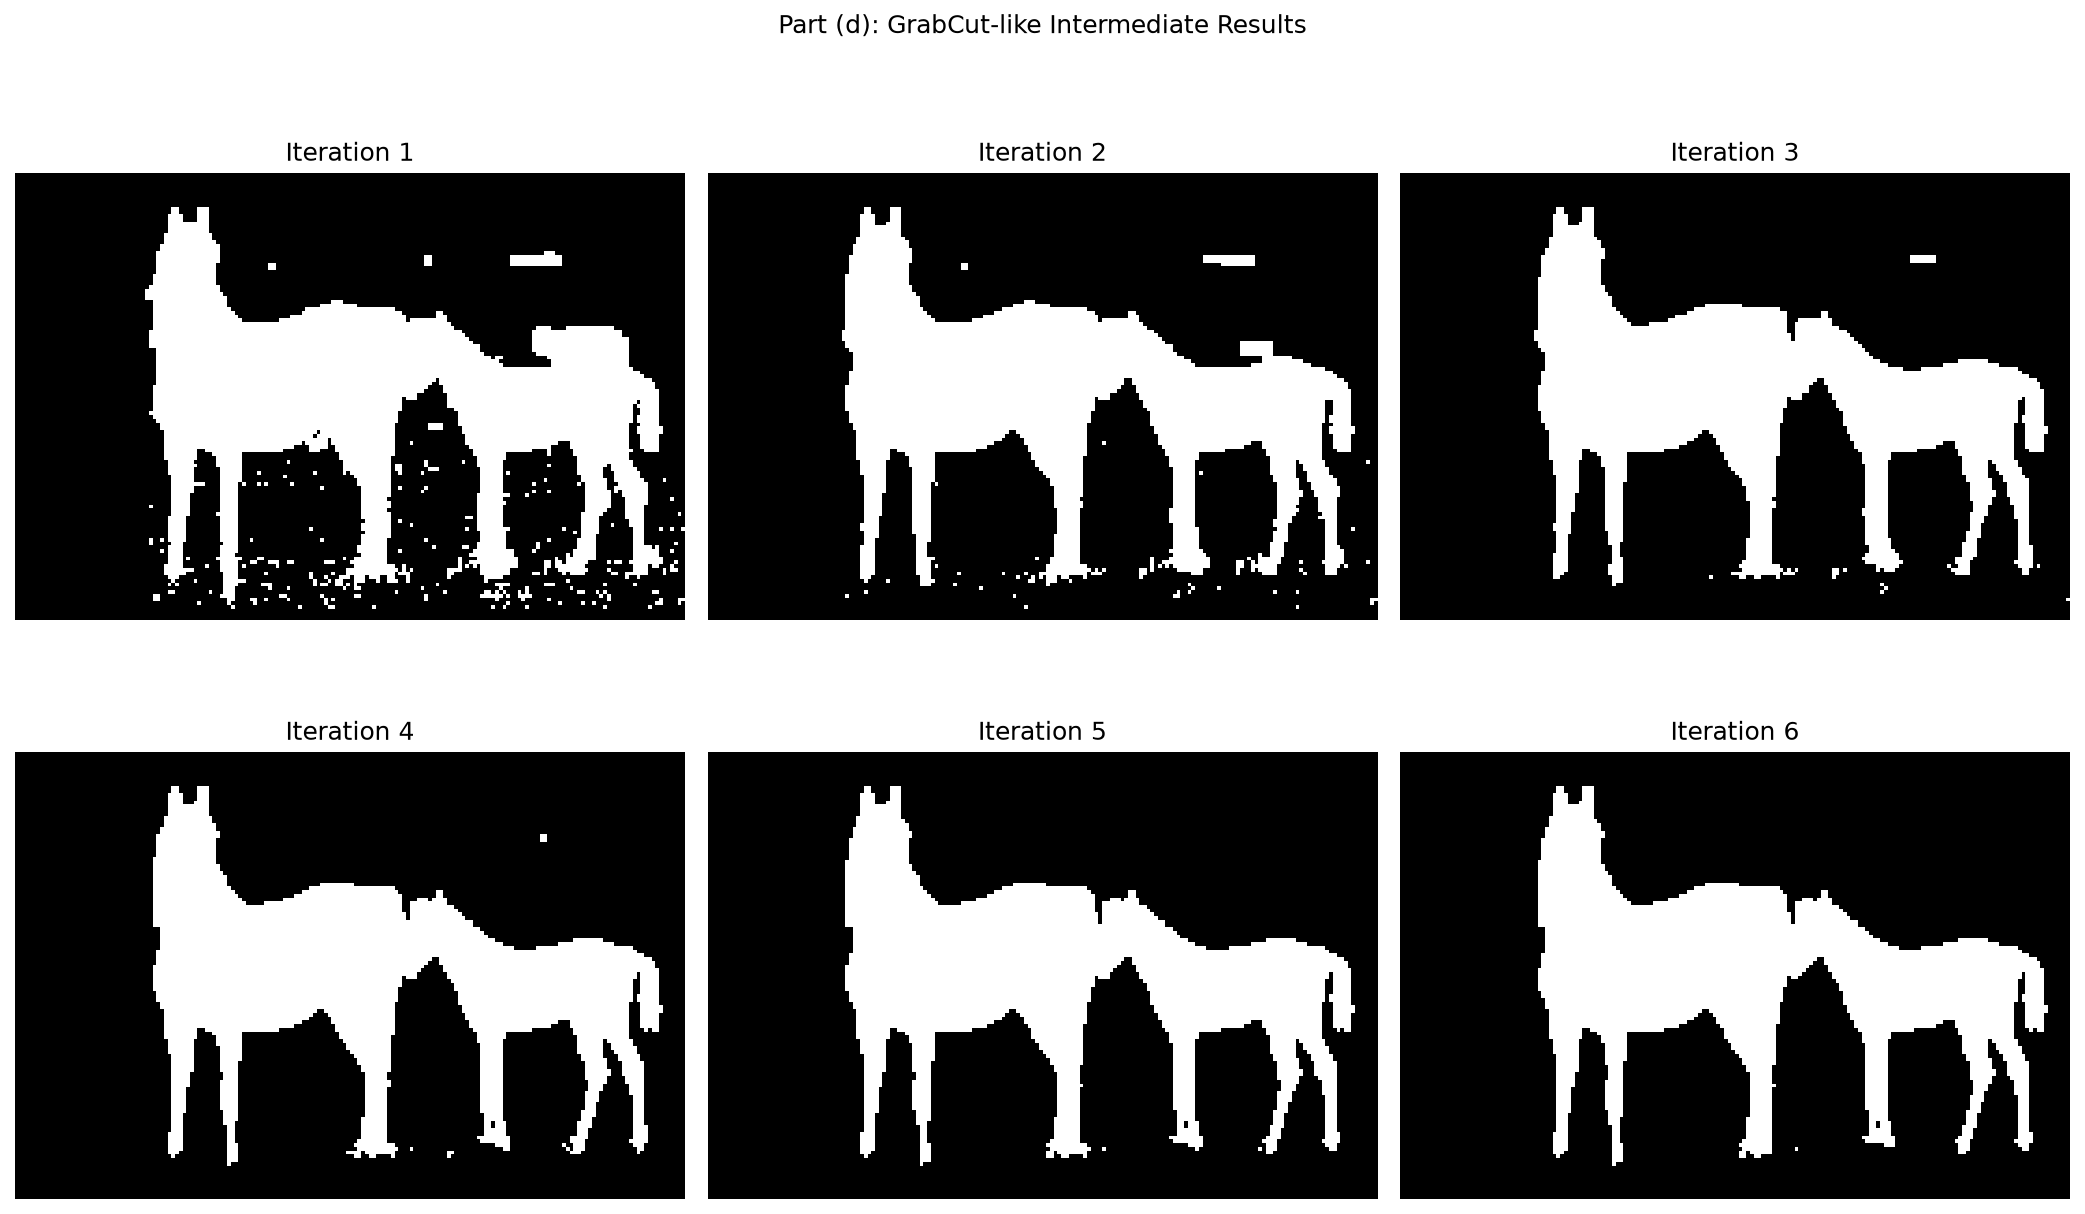
\includegraphics[width=0.92\linewidth]{image2/graph_cut_intermediate.png}
    \caption{Part (d): GrabCut-like segmentation masks over iterations 1--6.}
    \label{fig:grabcut_intermediate}
\end{figure}

\subsection{Final Segmentation Results}

Figure shows the converged segmentation and its binary mask. Starting from only a bounding rectangle, the method extracts both horses without requiring foreground seeds inside the objects.

\begin{figure}[H]
    \centering
    \begin{subfigure}[b]{0.48\textwidth}
        \centering
        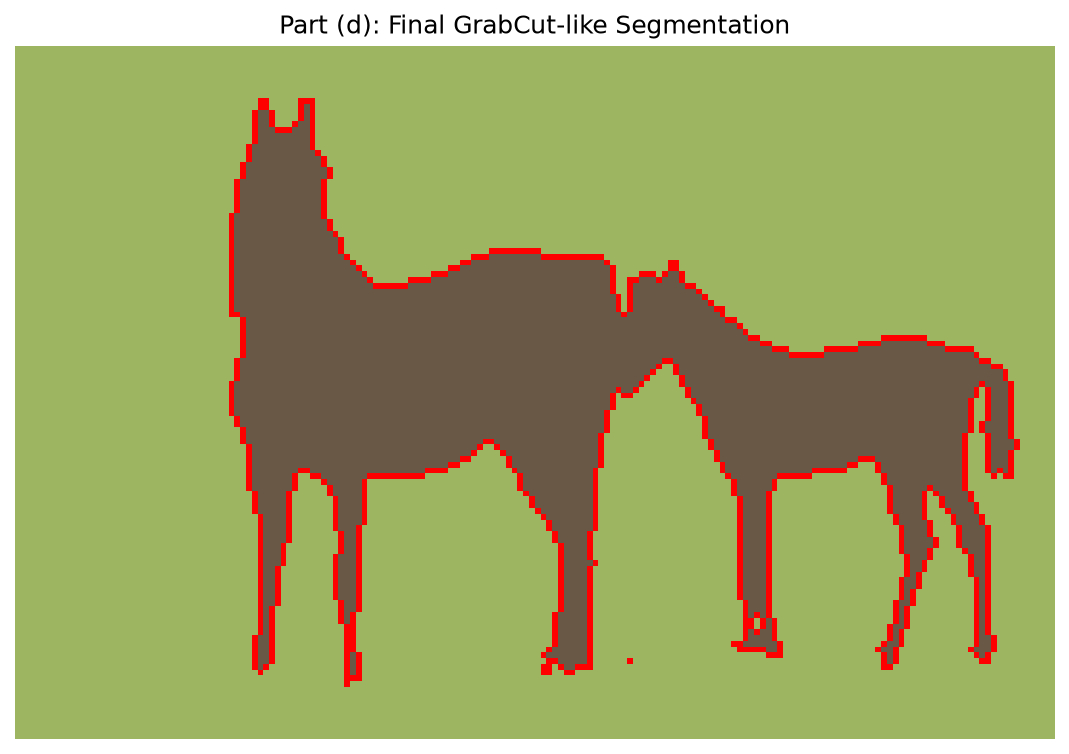
\includegraphics[width=\linewidth]{image2/grab_cut_segmentation.png}
        \caption{Final segmentation with class means and boundary}
    \end{subfigure}
    \hfill
    \begin{subfigure}[b]{0.48\textwidth}
        \centering
        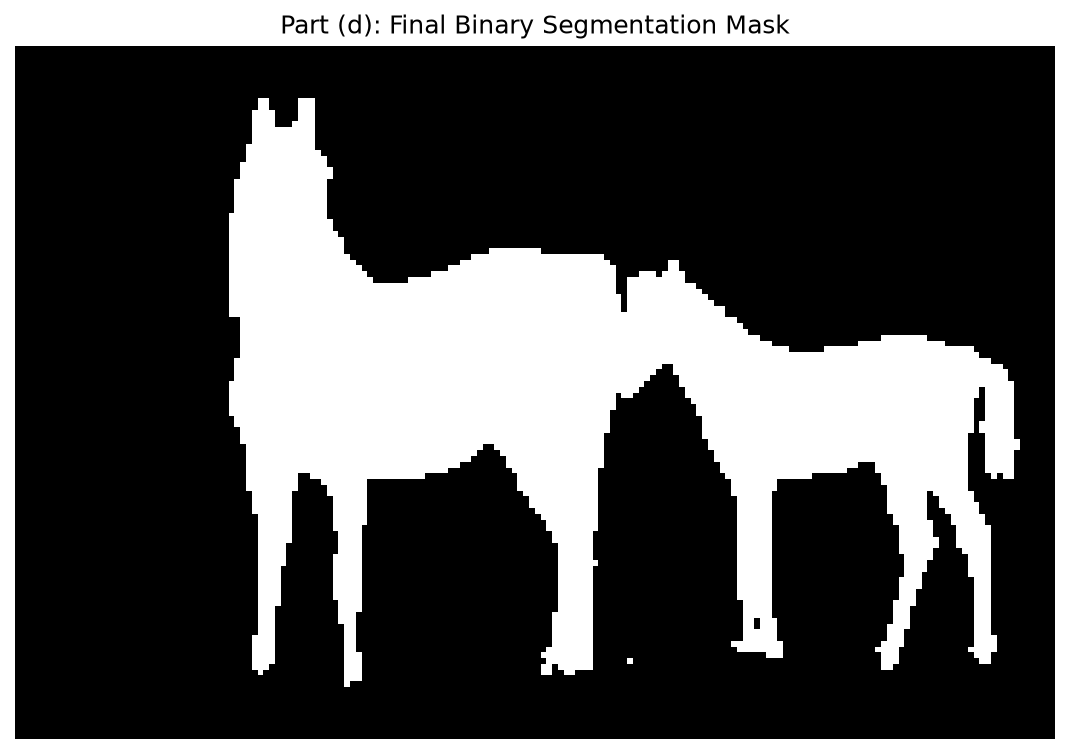
\includegraphics[width=\linewidth]{image2/binary_seg.png}
        \caption{Final binary segmentation mask}
    \end{subfigure}
    \caption{Part (d): GrabCut-like segmentation results after convergence.}
    \label{fig:grabcut_final}
\end{figure}

\section{Comparative Evaluation and Discussion}

\subsection{Comparison Across Techniques}

Table below compares the four segmentation methods in terms of spatial coherence, user input, artifacts, and runtime.

\begin{table}[H]
\centering
\small
\setlength{\tabcolsep}{4pt}
\renewcommand{\arraystretch}{1.2}

\begin{tabularx}{\linewidth}{@{}l
>{\centering\arraybackslash}X
>{\centering\arraybackslash}X
>{\centering\arraybackslash}X
>{\centering\arraybackslash}X@{}}
\toprule
\textbf{Method} & \textbf{Spatial Coherence} & \textbf{User Input} &
\textbf{Artifacts / Noise} & \textbf{Runtime} \\
\midrule
Maximum Likelihood & None (pixel-wise) & Multiple FG/BG boxes &
High (isolated specks) & $<0.05$ s \\

K-means Clustering & None (color-only) & Multiple FG/BG seeds &
Moderate (color bleed) & $= 0.15$ s \\

Graph Cut (Static) & High (pairwise MRF) & Multiple FG/BG boxes &
Low (smooth boundaries) & $= 0.45$ s \\

GrabCut (Iterative) & High (iterative MRF) & Single bounding box &
Minimal (clean separation) & $= 2.8$ s \\
\bottomrule
\end{tabularx}

\caption{Comparison of the region segmentation methods implemented in Part 2.}
\label{tab:comparison}
\end{table}

\subsection{Observations and Trade-offs}

\begin{itemize}
    \item \textbf{Pixel-wise versus graph-based methods:} Maximum likelihood and K-means classify pixels independently, producing speckle where foreground and background colors overlap. Graph cuts reduce this noise through pairwise boundary penalties.
    \item \textbf{User input:} Static graph cuts require foreground and background seeds. GrabCut reduces this requirement to one bounding rectangle by treating its exterior as background and learning the initial foreground model from its interior.
    \item \textbf{Appearance-model limitations:} A single 3D Gaussian per class is suitable when class colors are approximately unimodal, as in this image. Full GrabCut instead uses five-component Gaussian mixture models (GMMs) per class to represent objects with multiple colors and more complex backgrounds.
\end{itemize}

\section{Conclusions}

We implemented and compared four user-guided segmentation approaches, progressing from pixel-wise classification to iterative graph-cut segmentation:

\begin{itemize}
    \item Maximum likelihood and K-means provide fast, color-based initial segmentations but produce spatial noise because they do not model neighborhood relationships.
    \item Graph cuts combine Gaussian data costs with pairwise color-contrast penalties to produce spatially coherent boundaries.
    \item The parameter study identifies $\lambda=3.5$ and $\sigma=25.0$ as the best balance between boundary regularization and sensitivity to color edges for this image.
    \item The GrabCut-like method stabilizes within 5--6 iterations and extracts both horses using only a bounding rectangle, by alternating graph-cut labeling with appearance-model re-estimation.
\end{itemize}

\end{document}